\section{Ergebnisse}

\subsection{Modellvergleich}

\begin{table}[H]
  \centering
  \footnotesize
  \begin{tabular}{lrrrrr}
    \toprule
    Modell & F1 & ROC-AUC & PR-AUC & Precision & Recall \\
    \midrule
    Trivial (Mehrheitskl.) (ohne SMOTE) & $0,000 \pm 0,000$ & 0,500 & 0,261 & 0,000 & 0,000 \\
    Trivial (Mehrheitskl.) (mit SMOTE) & $0,000 \pm 0,000$ & 0,500 & 0,261 & 0,000 & 0,000 \\
    Log. Regression (ohne SMOTE) & $0,630 \pm 0,095$ & 0,851 & 0,706 & 0,533 & 0,781 \\
    Log. Regression (mit SMOTE) & $0,631 \pm 0,107$ & 0,853 & 0,706 & 0,536 & 0,775 \\
    Random Forest (ohne SMOTE) & $0,609 \pm 0,081$ & 0,819 & 0,635 & 0,538 & 0,711 \\
    Random Forest (mit SMOTE) & $0,589 \pm 0,083$ & 0,813 & 0,610 & 0,535 & 0,668 \\
    Gradient Boosting (ohne SMOTE) & $0,553 \pm 0,086$ & 0,816 & 0,639 & 0,648 & 0,487 \\
    Gradient Boosting (mit SMOTE) & $0,593 \pm 0,109$ & 0,816 & 0,619 & 0,580 & 0,618 \\
    Neuronales Netz (ohne SMOTE) & $0,496 \pm 0,100$ & 0,807 & 0,619 & 0,569 & 0,448 \\
    Neuronales Netz (mit SMOTE) & $0,581 \pm 0,085$ & 0,792 & 0,595 & 0,518 & 0,667 \\
    \bottomrule
  \end{tabular}
\end{table}


Das beste Ergebnis erzielt \textbf{Logistische Regression + SMOTE} mit F1 = 0,631
($\pm$ 0,107) und ROC-AUC = 0,853.

\begin{figure}[H]
  \centering
  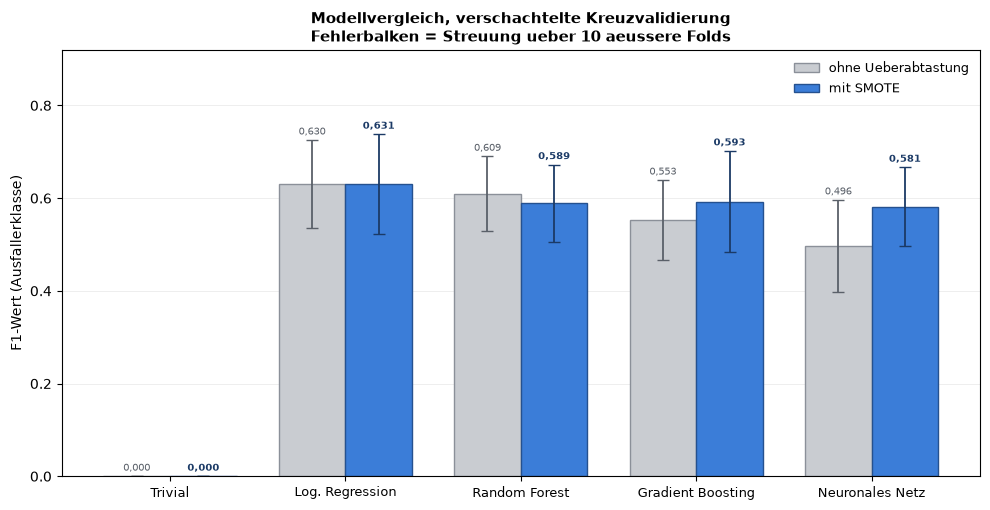
\includegraphics[width=0.90\linewidth]{05_modellvergleich_f1.png}
  \caption{F1-Wert je Verfahren, ohne und mit Ueberabtastung. Fehlerbalken: Streuung ueber die zehn aeusseren Folds.}
\end{figure}


\textbf{Die Modelle ordnen die Kunden deutlich besser, als der F1-Wert
vermuten laesst.} Ein ROC-AUC-Wert von 0,853 bedeutet:
Zieht man einen zufaelligen Ausfaller und einen zufaelligen Nicht-Ausfaller
heraus, wird der Ausfaller in rund 85,3~\% der
Faelle hoeher eingestuft. Der niedrigere F1-Wert entsteht allein durch die
feste Schwelle 0,5 -- dazu Abschnitt~\ref{sec:schwelle}.

\subsection{Bringt Ueberabtastung etwas?}

Fuer die logistische Regression ist der Unterschied nicht unterscheidbar (p = 0,844),
fuer das neuronale Netz signifikant (p = 0,037),
fuer den Random Forest signifikant (p = 0,039).
Ob SMOTE hilft, haengt also von der Konfiguration ab und ist keine allgemeine
Regel.

\subsection{Treiber des Ausfalls}

Standardisierte Koeffizienten der logistischen Regression (untereinander
vergleichbar, weil alle Merkmale dieselbe Skala haben), mit
Bootstrap-Konfidenzintervall und Permutationswichtigkeit (Abfall der ROC-AUC
beim zufaelligen Durchmischen des Merkmals):

\begin{table}[H]
  \centering
  \footnotesize
  \begin{tabular}{lrrrll}
    \toprule
    Merkmal & Koeffizient & Odds-Ratio & KI95 & signifikant & Perm.-AUC \\
    \midrule
    Beschaeftigungsjahre & -1,61 & 0,20 & [-2,07; -1,26] & ja & 0,126 \\
    Kreditkartenschuld & 1,21 & 3,36 & [0,85; 1,69] & ja & 0,039 \\
    Wohnjahre an der Adresse & -0,66 & 0,52 & [-1,04; -0,36] & ja & 0,010 \\
    Schulden-Einkommens-Quote & 0,51 & 1,67 & [0,17; 0,88] & ja & 0,061 \\
    Einkommen (Tsd.) & -0,29 & 0,75 & [-0,85; 0,14] & nein & 0,005 \\
    Alter & 0,27 & 1,31 & [-0,00; 0,53] & nein & 0,007 \\
    Sonstige Schulden & 0,12 & 1,12 & [-0,29; 0,53] & nein & 0,010 \\
    Bildungsstufe & 0,11 & 1,12 & [-0,10; 0,31] & nein & 0,010 \\
    \bottomrule
  \end{tabular}
\end{table}


Die Schulden-Einkommens-Quote und die Kreditkartenschuld erhoehen das Risiko,
Beschaeftigungsjahre und Wohnjahre senken es. Ein Odds-Ratio von
1,67 bei der Schuldenquote heisst: Eine
Erhoehung um eine Standardabweichung vervielfacht die Chance auf einen Ausfall
etwa um diesen Faktor. Einkommen, Alter, sonstige Schulden und Bildungsstufe
sind im Modell \emph{nicht} von Null unterscheidbar.

\begin{figure}[H]
  \centering
  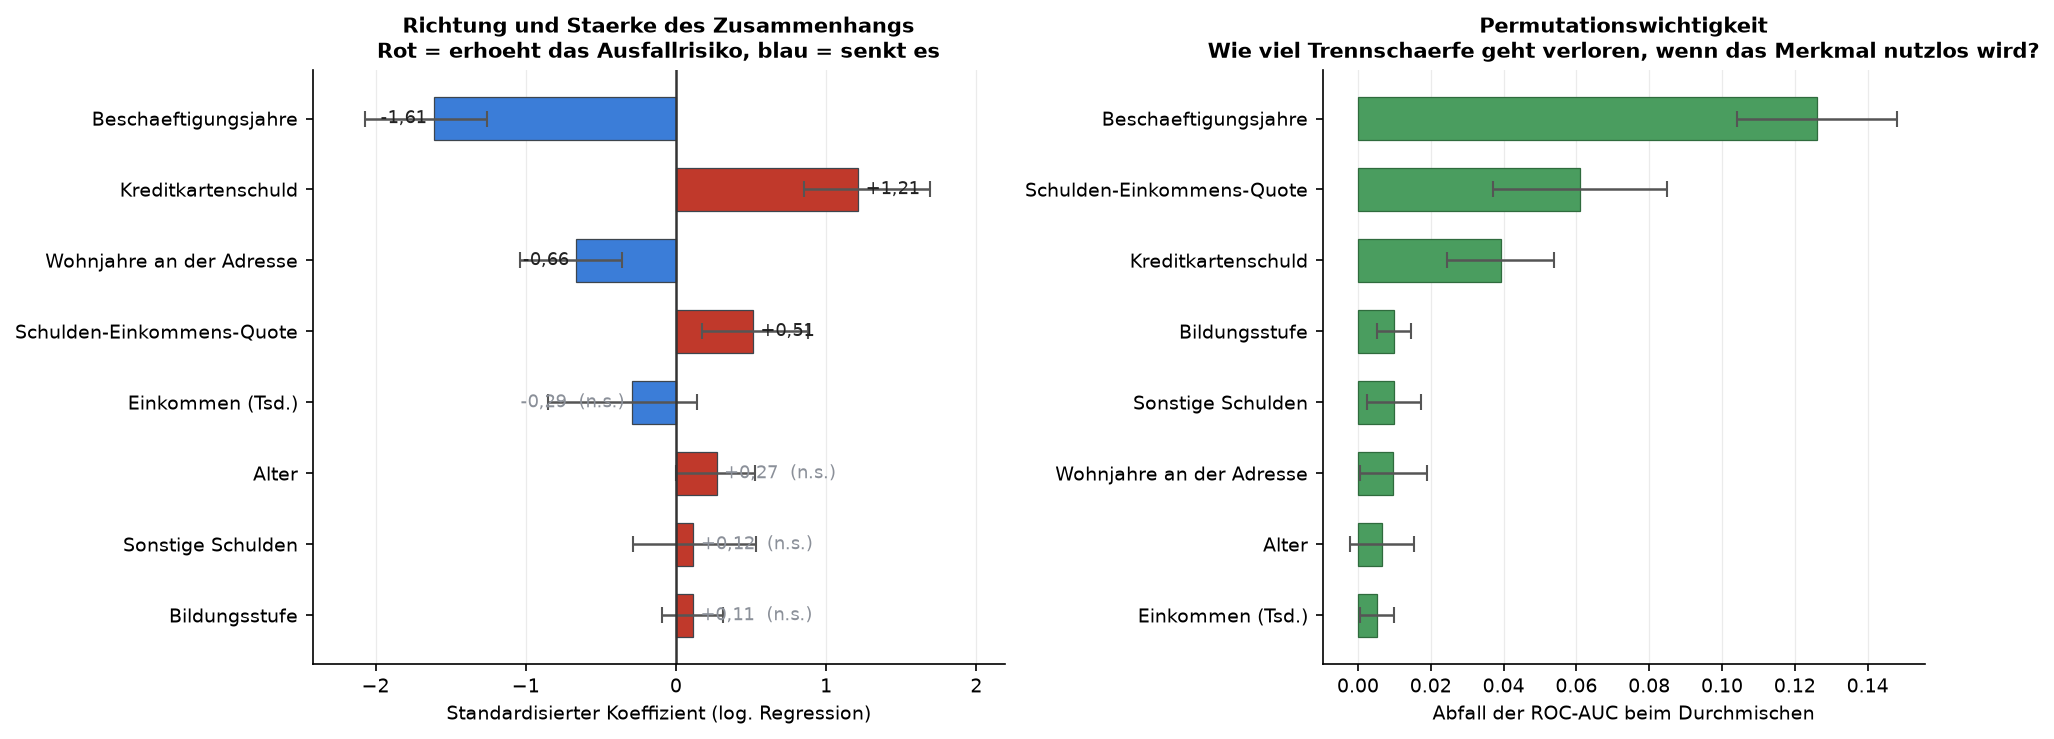
\includegraphics[width=0.90\linewidth]{06_treiber.png}
  \caption{Links: Richtung und Staerke des Zusammenhangs (standardisiert). Rechts: wie viel Trennschaerfe verloren geht, wenn ein Merkmal nutzlos gemacht wird.}
\end{figure}

